\documentclass[11pt,twocolumn]{article}

% ─── Packages ───────────────────────────────────────────────────────────────
\usepackage{fix-cm}
\usepackage[T1]{fontenc}
\usepackage[margin=1in]{geometry}
\usepackage{amsmath,amssymb}
\usepackage{booktabs}
\usepackage{tabularx}
\usepackage{listings}
\usepackage{xcolor}
\usepackage{hyperref}
\usepackage{graphicx}
\usepackage{caption}
\usepackage{subcaption}
\usepackage{enumitem}
\usepackage{titlesec}
\usepackage{fancyhdr}
\usepackage{parskip}
\usepackage{tikz}
\usetikzlibrary{shapes.geometric, arrows.meta, positioning, fit, backgrounds}
\usepackage{array}
\usepackage{multirow}
\usepackage{url}
\usepackage[numbers]{natbib}
\usepackage{pgfplots}
\pgfplotsset{compat=1.18}
\usepackage{algorithm}
\usepackage{algorithmic}

% ─── Colours ────────────────────────────────────────────────────────────────
\definecolor{codeblue}{rgb}{0.08,0.38,0.74}
\definecolor{codegray}{rgb}{0.5,0.5,0.5}
\definecolor{codegreen}{rgb}{0.13,0.55,0.13}
\definecolor{codebg}{rgb}{0.97,0.97,0.97}
\definecolor{accentblue}{rgb}{0.08,0.38,0.74}

% ─── Code listings ──────────────────────────────────────────────────────────
\lstdefinestyle{typescript}{
  backgroundcolor=\color{codebg},
  commentstyle=\color{codegreen}\itshape,
  keywordstyle=\color{codeblue}\bfseries,
  stringstyle=\color{orange},
  basicstyle=\ttfamily\footnotesize,
  breakatwhitespace=false,
  breaklines=true,
  keepspaces=true,
  numbers=left,
  numbersep=5pt,
  numberstyle=\tiny\color{codegray},
  showspaces=false,
  showstringspaces=false,
  tabsize=2,
  frame=single,
  framerule=0.4pt,
  rulecolor=\color{codegray},
}
\lstset{style=typescript}

% ─── Section formatting ─────────────────────────────────────────────────────
\titleformat{\section}{\large\bfseries\color{accentblue}}{\thesection.}{0.5em}{}
\titleformat{\subsection}{\normalsize\bfseries}{\thesubsection.}{0.5em}{}
\titleformat{\subsubsection}{\normalsize\itshape}{\thesubsubsection.}{0.5em}{}

% ─── Headers / footers ──────────────────────────────────────────────────────
\pagestyle{fancy}
\fancyhf{}
\renewcommand{\headrulewidth}{0.4pt}
\fancyhead[L]{\footnotesize\textit{Pointer-Based Agent Memory}}
\fancyhead[R]{\footnotesize\textit{Tham, 2026}}
\fancyfoot[C]{\thepage}

% ─── Hyperref setup ─────────────────────────────────────────────────────────
\hypersetup{
  colorlinks=true,
  linkcolor=accentblue,
  citecolor=accentblue,
  urlcolor=accentblue,
  pdftitle={Entity-Learn: Zero-Copy Live Memory for Autonomous Agents via Command Pointer Replay},
  pdfauthor={Lewis Tham},
}

% ─── Misc ────────────────────────────────────────────────────────────────────
\setlength{\columnsep}{0.25in}

% ═════════════════════════════════════════════════════════════════════════════
\begin{document}

\title{\textbf{Entity-Learn: Zero-Copy Live Memory for Autonomous Agents}\\[6pt]
\large\textit{Command Pointer Replay, Auto-Schema Inference, and Cross-Source BM25 Retrieval}}

\author{%
  Lewis Tham\\[6pt]
  Unbrowse AI \quad \texttt{lewis@unbrowse.ai}
}

\date{}
\maketitle
\thispagestyle{fancy}

% ─── Abstract ────────────────────────────────────────────────────────────────
\begin{abstract}
Existing memory systems for LLM agents copy data into dedicated stores---vector databases, knowledge graphs, or structured files---creating a fundamental tension between freshness and fidelity.
We present \textbf{Entity-Learn}, a \emph{zero-copy} memory architecture that stores only \emph{command pointers}---the shell commands or API calls that produce data---and replays them at query time to obtain live results.
Entity-Learn automatically infers entity schemas (type, ID field, title field, status field) from JSON output without any LLM call, discovers cross-entity relations through pattern matching, and ranks results across heterogeneous sources using BM25.
A bootstrap mechanism mines prior agent session histories for recurring data-producing commands, auto-populating the pointer store from real usage patterns.
The entire system requires zero external infrastructure---no vector database, no graph database, no embedding service---with all state stored in a single 31.9\,KB JSON file.
In a production deployment spanning 50 pointers across 31 entity types, Entity-Learn resolves 400 entities from 7 data source categories, discovers 525 cross-entity relations (79\% of entities linked), and serves warm queries in 57--128\,ms.
A single \texttt{bootstrap} invocation mines 200 agent session files in 0.69\,s, discovering 32 new data-producing commands across analytics, CRM, email, messaging, and code hosting APIs.

\medskip
\noindent\textbf{Keywords:} Agent memory, Zero-copy architecture, Command pointers, Schema inference, BM25, Cross-source retrieval, Session history mining, LLM agents
\end{abstract}

% ═════════════════════════════════════════════════════════════════════════════
\section{Introduction}
\label{sec:intro}

The rise of autonomous LLM agents that operate across multiple tools and data sources has created an urgent need for persistent memory.
An agent debugging a software issue may need to correlate a GitHub issue with an email thread, a CRM record, and a deployment log---all from different APIs, all changing in real time.

Current approaches to agent memory fall into three categories:
(1)~\emph{snapshot stores} that copy data into vector databases or knowledge graphs~\cite{amem2025, zep2025, magma2026},
(2)~\emph{LLM-curated stores} that use the language model itself to structure and maintain knowledge~\cite{byterover2026, memos2025},
and (3)~\emph{session buffers} that maintain working memory within a conversation~\cite{memtool2025, memoryr1_2025}.

All three share a fundamental limitation: they store \emph{data}, not \emph{access patterns}.
The moment data is copied, it begins to decay.
A GitHub issue's status changes, a CRM deal advances, an email thread grows---and the stored snapshot diverges from reality.
Systems compensate with periodic refresh, change detection, or TTL-based invalidation, but these add complexity and can never guarantee freshness at query time.

We propose a different primitive: \textbf{the command pointer}.
Instead of copying the result of \texttt{gh api repos/org/repo/issues}, Entity-Learn stores the command itself along with an auto-inferred schema of its output.
At query time, the command is re-executed, producing live data that is immediately shaped, ranked, and linked to entities from other sources.

This \emph{zero-copy} approach yields five properties that distinguish Entity-Learn from all prior work:

\begin{enumerate}[leftmargin=1.5em,itemsep=2pt]
  \item \textbf{Guaranteed freshness.} Data is fetched at query time, not at storage time. There is no staleness window.
  \item \textbf{Zero infrastructure.} No vector database, no graph database, no embedding model. The entire state is a single JSON file.
  \item \textbf{Automatic schema inference.} Entity types, ID fields, title fields, and status fields are inferred from JSON output without any LLM call.
  \item \textbf{Session history mining.} A bootstrap mechanism scans prior agent sessions for recurring data-producing commands, auto-populating the pointer store.
  \item \textbf{Cross-source retrieval.} BM25 ranking across heterogeneous entity types enables unified search without embeddings.
\end{enumerate}

Entity-Learn is deployed in production as a skill for Claude Code agents, where it manages 30+ entity types across GitHub, Gmail, Google Calendar, CRM systems, analytics endpoints, and local JSON files.


% ═════════════════════════════════════════════════════════════════════════════
\section{Related Work}
\label{sec:related}

\subsection{Snapshot-Based Memory}

A-MEM~\cite{amem2025} applies the Zettelkasten method to agent memory, creating interconnected knowledge networks through dynamic indexing.
Zep~\cite{zep2025} builds a temporal knowledge graph (Graphiti) that synthesizes conversational and structured data while maintaining historical relationships.
MAGMA~\cite{magma2026} uses multi-graph architectures to record interaction histories.
All three copy data into dedicated stores, creating a freshness-fidelity tradeoff.

The ``Hindsight'' system~\cite{hindsight2025} combines BM25 lexical search with semantic retrieval over stored memories, achieving strong recall on proper nouns and technical terms.
Entity-Learn shares the BM25 component but eliminates the storage layer entirely.

\subsection{LLM-Curated Memory}

ByteRover~\cite{byterover2026} is the closest work to ours in philosophy: it stores knowledge as human-readable markdown files with no external infrastructure.
However, ByteRover still copies data---the LLM curates \emph{what} to store, but stores it nonetheless.
Entity-Learn inverts this: it stores \emph{how to get the data}, not the data itself.

MemOS~\cite{memos2025} proposes a memory operating system with full lifecycle management (creation, activation, fusion, disposal), treating memory as a managed system resource.
While architecturally elegant, MemOS requires substantial infrastructure and does not address the freshness problem.

\subsection{Tool Memory and Procedural Memory}

MemTool~\cite{memtool2025} addresses tool management in multi-turn conversations, pruning and persisting available tools across sessions.
This is complementary to Entity-Learn: MemTool manages \emph{which tools} are available; Entity-Learn manages \emph{what data those tools produce}.

Mem$^p$~\cite{memp2025} explores procedural memory---compiling habitual skills into executable subroutines.
Entity-Learn's bootstrap mechanism is conceptually similar: it mines session histories for recurring data-access patterns and compiles them into reusable pointers.

Memory-R1~\cite{memoryr1_2025} uses reinforcement learning to train a memory manager on structured operations (ADD, UPDATE, DELETE).
Entity-Learn's learn/query interface serves a similar role but operates without any training, using heuristic schema inference instead.

\subsection{Surveys}

``Memory in the Age of AI Agents''~\cite{memsurvey2025} provides a comprehensive taxonomy, identifying fragmentation across motivations, implementations, and evaluation protocols.
The Structured Distillation work~\cite{structdistill2026} achieves 11$\times$ token reduction while preserving retrieval quality through BM25 indexing.
Both validate the design choices in Entity-Learn: lightweight retrieval (BM25 over embeddings) and minimal storage overhead.


% ═════════════════════════════════════════════════════════════════════════════
\section{System Design}
\label{sec:design}

Entity-Learn has four components: \textbf{Learn} (pointer creation with schema inference), \textbf{Resolve} (live data fetching with caching), \textbf{Query} (cross-source BM25 retrieval with relation discovery), and \textbf{Bootstrap} (session history mining).

\subsection{Architecture Overview}

\begin{figure*}[t]
\centering
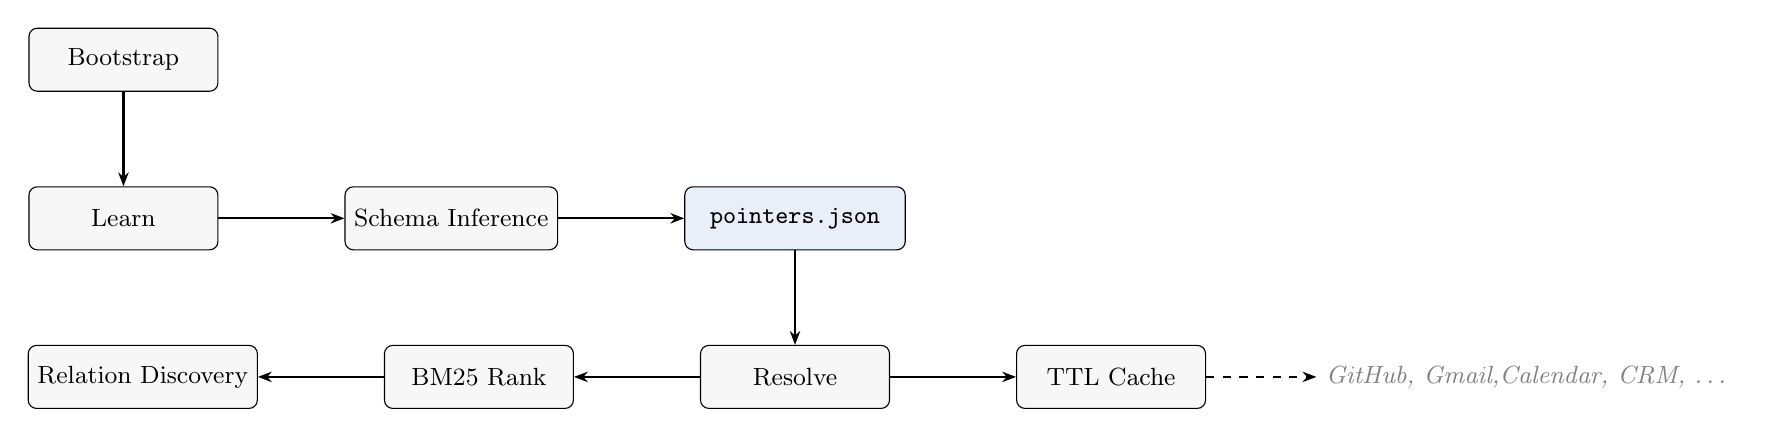
\begin{tikzpicture}[
  node distance=1.2cm and 1.6cm,
  box/.style={draw, rounded corners=3pt, minimum width=2.4cm, minimum height=0.8cm, font=\small, fill=codebg},
  store/.style={draw, rounded corners=3pt, minimum width=2.8cm, minimum height=0.8cm, font=\small, fill=accentblue!10},
  arrow/.style={-{Stealth[length=5pt]}, thick},
]

% Nodes
\node[box] (learn) {Learn};
\node[box, right=of learn] (schema) {Schema Inference};
\node[store, right=of schema] (store) {\texttt{pointers.json}};
\node[box, below=of store] (resolve) {Resolve};
\node[box, left=of resolve] (bm25) {BM25 Rank};
\node[box, left=of bm25] (relations) {Relation Discovery};
\node[box, above=of learn] (bootstrap) {Bootstrap};
\node[box, right=of resolve] (cache) {TTL Cache};

% External
\node[right=1.4cm of cache, font=\small\itshape, text=codegray] (apis) {GitHub, Gmail,\\Calendar, CRM, \ldots};

% Arrows
\draw[arrow] (learn) -- (schema);
\draw[arrow] (schema) -- (store);
\draw[arrow] (store) -- (resolve);
\draw[arrow] (resolve) -- (bm25);
\draw[arrow] (bm25) -- (relations);
\draw[arrow] (bootstrap) -- (learn);
\draw[arrow] (resolve) -- (cache);
\draw[arrow, dashed] (cache) -- (apis);

\end{tikzpicture}
\caption{Entity-Learn architecture. The pointer store holds only command strings and inferred schemas. At query time, \texttt{Resolve} re-executes commands (with TTL caching) to obtain live data, which is then ranked by BM25 and linked through relation discovery. Bootstrap auto-populates pointers from session history.}
\label{fig:architecture}
\end{figure*}

The entire ``database'' is a single JSON file (\texttt{\textasciitilde/.agent-org/pointers.json}) containing an array of \emph{Pointer} records and a TTL-based cache.
A Pointer stores:

\begin{itemize}[leftmargin=1.5em,itemsep=1pt]
  \item \texttt{command}: the shell command that produces data
  \item \texttt{entity\_type}: auto-inferred or user-specified type label
  \item \texttt{result\_shape}: \texttt{array}, \texttt{object}, or \texttt{object\_of\_objects}
  \item \texttt{id\_field}, \texttt{title\_field}, \texttt{status\_field}: auto-detected field names
  \item \texttt{fields}: list of primitive fields in the output schema
  \item \texttt{confidence}: inference confidence score (0--1)
  \item \texttt{ttl\_seconds}: cache duration (default 300s)
  \item Usage statistics: \texttt{use\_count}, \texttt{last\_used}, \texttt{learned\_at}
\end{itemize}

\subsection{Learn: Pointer Creation with Schema Inference}
\label{sec:learn}

When an agent encounters a useful data-producing command, it invokes \texttt{entity-learn learn "command"}.
The system:

\begin{enumerate}[leftmargin=1.5em,itemsep=2pt]
  \item \textbf{Executes} the command and captures its stdout.
  \item \textbf{Parses} the output as JSON. Non-JSON output is rejected.
  \item \textbf{Detects result shape}: array of objects, single object, or object-of-objects (a dictionary where each value is itself an object).
  \item \textbf{Infers entity type} from the command string using segment analysis (e.g., \texttt{gh api repos/.../issues} $\rightarrow$ \texttt{issue}).
  \item \textbf{Infers key fields} by matching JSON keys against ranked candidate lists:
    \begin{itemize}[leftmargin=1em,itemsep=0pt]
      \item ID: \texttt{id}, \texttt{number}, \texttt{\_id}, \texttt{key}, \texttt{slug}, \texttt{login}, \ldots
      \item Title: \texttt{title}, \texttt{name}, \texttt{subject}, \texttt{summary}, \texttt{description}, \ldots
      \item Status: \texttt{status}, \texttt{state}, \texttt{stage}, \texttt{phase}, \texttt{priority}, \ldots
    \end{itemize}
  \item \textbf{Computes confidence}: $c = 0.5 + 0.2 \cdot \mathbb{1}[\text{id found}] + 0.2 \cdot \mathbb{1}[\text{title found}] + 0.1 \cdot \mathbb{1}[\text{status found}]$.
  \item \textbf{Stores} the pointer. If a pointer for the same command exists, it is updated rather than duplicated.
\end{enumerate}

The key insight is that schema inference operates on a small sample (5 items) and uses only string matching against known field-name conventions.
No LLM call is required, making the operation deterministic and sub-millisecond.

\begin{algorithm}[t]
\caption{Schema Inference}
\label{alg:schema}
\begin{algorithmic}[1]
\REQUIRE Command $c$, JSON output $J$
\ENSURE Pointer $p$ or $\bot$
\STATE $J \leftarrow \text{\textsc{Parse}}(c.\text{stdout})$
\IF{$J$ is array}
  \STATE $\text{shape} \leftarrow \texttt{array}$; $S \leftarrow J[0{:}5]$
\ELSIF{$J$ is object-of-objects}
  \STATE $\text{shape} \leftarrow \texttt{object\_of\_objects}$; $S \leftarrow \text{values}(J)[0{:}5]$
\ELSIF{$J$ is object}
  \STATE $\text{shape} \leftarrow \texttt{object}$; $S \leftarrow [J]$
\ELSE
  \RETURN $\bot$
\ENDIF
\STATE $K \leftarrow \bigcup_{s \in S} \text{keys}(s)$
\STATE $\text{id} \leftarrow \text{\textsc{Match}}(K, \text{ID\_CANDIDATES})$
\STATE $\text{title} \leftarrow \text{\textsc{Match}}(K, \text{TITLE\_CANDIDATES})$
\STATE $\text{status} \leftarrow \text{\textsc{Match}}(K, \text{STATUS\_CANDIDATES})$
\STATE $\text{type} \leftarrow \text{\textsc{InferType}}(c)$ \COMMENT{from command segments}
\STATE $\text{conf} \leftarrow 0.5 + 0.2[\text{id}] + 0.2[\text{title}] + 0.1[\text{status}]$
\RETURN $p(c, \text{type}, \text{shape}, \text{id}, \text{title}, \text{status}, K, \text{conf})$
\end{algorithmic}
\end{algorithm}


\subsection{Resolve: Live Data Fetching}
\label{sec:resolve}

When a query requires data from a pointer, \texttt{Resolve} checks the TTL cache first.
If the cached result is within \texttt{ttl\_seconds}, it is returned immediately.
Otherwise, the command is re-executed:

\begin{enumerate}[leftmargin=1.5em,itemsep=2pt]
  \item Execute the stored command with a 30-second timeout.
  \item Parse the JSON output.
  \item Update the cache entry with a fresh timestamp.
  \item Increment the pointer's \texttt{use\_count} and \texttt{last\_used}.
  \item On failure, return stale cache if available; otherwise \texttt{null}.
\end{enumerate}

For pageable commands (those with \texttt{per\_page}, \texttt{limit}, or \texttt{pageSize} parameters), Resolve supports pagination by appending \texttt{\&page=N} to the command URL.

The TTL cache provides a crucial optimization: during a single agent session, multiple queries to the same entity type reuse cached results.
The default TTL of 300 seconds balances freshness against API rate limits.
Stale-on-error fallback ensures graceful degradation when upstream services are temporarily unavailable.


\subsection{Query: Cross-Source BM25 Retrieval}
\label{sec:query}

Entity-Learn's query system resolves all matching pointers, normalizes the results into a uniform entity representation, ranks them with BM25, and optionally discovers cross-entity relations.

\subsubsection{Entity Normalization}

Each resolved JSON result is transformed into a \texttt{ResolvedEntity}:

\begin{lstlisting}[language=Java,caption={ResolvedEntity structure}]
interface ResolvedEntity {
  id: string;
  type: string;        // e.g., "issue", "email"
  title: string;       // from title_field
  status?: string;     // from status_field
  source_command: string;
  data: Record<string, unknown>;
  related?: Relation[];
}
\end{lstlisting}

The normalization handles three result shapes uniformly: arrays yield one entity per element; objects yield a single entity; objects-of-objects yield one entity per value, using the key as the ID.

\subsubsection{BM25 Ranking}

Given a query string $q$, we tokenize $q$ and each entity's concatenated text (title + type + status + all string field values) into token sets.
The standard BM25 scoring function ranks entities:

\begin{equation}
\text{score}(e, q) = \sum_{t \in q} \text{IDF}(t) \cdot \frac{f(t, e) \cdot (k_1 + 1)}{f(t, e) + k_1 \cdot (1 - b + b \cdot |e| / \overline{|e|})}
\end{equation}

where $f(t, e)$ is the term frequency of $t$ in entity $e$, $|e|$ is the document length, $\overline{|e|}$ is the average document length across all entities, and we use $k_1 = 1.5$, $b = 0.75$ (standard defaults).

BM25 is particularly effective for agent memory because agent queries tend to contain specific identifiers (issue numbers, email addresses, project names) where exact lexical matching outperforms semantic similarity.

\subsubsection{Cross-Entity Relation Discovery}
\label{sec:relations}

After resolving and ranking, Entity-Learn discovers relations between entities through five pattern-matching strategies:

\begin{enumerate}[leftmargin=1.5em,itemsep=2pt]
  \item \textbf{Email matching}: Entities sharing email addresses (regex-extracted from all string fields).
  \item \textbf{ID references}: Values matching patterns like \texttt{\#123}, \texttt{issue/456}, or prefixed identifiers.
  \item \textbf{Version tags}: Shared version strings (e.g., \texttt{v1.2.3}).
  \item \textbf{Name matching}: Shared person or organization names across entity types.
  \item \textbf{Value overlap}: Any distinctive string value (3--60 chars, excluding URLs, dates, and common status words) appearing in 2--8 entities.
\end{enumerate}

Relations are indexed using an inverted map: for each linkable value, we track which entities contain it.
Two entities sharing a value are linked.
Values appearing in more than 8 entities are considered non-distinctive and excluded.
Each entity retains at most 10 relations.

This approach discovers relations like ``this GitHub issue was filed by the same person who sent this email'' or ``this CRM deal references the same company as this calendar event'' without any explicit graph construction.


\subsection{Bootstrap: Session History Mining}
\label{sec:bootstrap}

The bootstrap mechanism scans Claude Code session history (\texttt{\textasciitilde/.claude/projects/} JSONL files) for Bash tool calls that:

\begin{enumerate}[leftmargin=1.5em,itemsep=2pt]
  \item Match data-producing patterns (48 regex patterns covering \texttt{gh api}, \texttt{curl}, \texttt{gws}, \texttt{jq}, and API-specific URLs).
  \item Were used at least twice across sessions (frequency threshold filters noise from one-off exploratory commands).
  \item Do not already exist as pointers.
  \item Do not match skip patterns (localhost, health checks, write operations).
\end{enumerate}

Commands are normalized by stripping variable substitutions and pipe chains, then deduplicated by \texttt{(type, normalized\_command)} key.
The most frequently used commands are taught first.

Bootstrap effectively extracts the agent's implicit data-access knowledge---the commands it has learned to use for specific entity types---and compiles it into explicit, reusable pointers.
A single \texttt{bootstrap} invocation typically discovers 30--50 entity types from 200 session files.


% ═════════════════════════════════════════════════════════════════════════════
\section{Formal Properties}
\label{sec:formal}

\subsection{Freshness Guarantee}

\begin{definition}[Data Freshness]
For a query at time $t_q$, let $t_d$ be the timestamp of the data returned. A memory system has \emph{staleness window} $\delta = t_q - t_d$.
\end{definition}

\begin{theorem}[Zero Staleness]
Entity-Learn's staleness window $\delta$ is bounded by the execution time of the underlying command: $\delta \leq t_{\text{exec}}$, where $t_{\text{exec}}$ is the wall-clock time of the command execution.
\end{theorem}

\begin{proof}
When the TTL cache is expired (or on first access), Resolve executes the command at time $t_q$, obtaining data timestamped at $t_q + t_{\text{exec}}$.
The returned data is therefore at most $t_{\text{exec}}$ old.
Since $t_{\text{exec}} < 30$s (the timeout bound), $\delta < 30$s.
\end{proof}

Snapshot-based systems have $\delta = t_q - t_{\text{snapshot}}$, which grows without bound unless a refresh mechanism is triggered.
Even with periodic refresh at interval $R$, $\delta \leq R$, and $R$ must be balanced against API rate limits and storage costs.

\subsection{Storage Complexity}

Let $n$ be the number of entity types and $k$ be the average number of fields per type.

\begin{itemize}[leftmargin=1.5em,itemsep=2pt]
  \item \textbf{Entity-Learn}: $O(n \cdot (|c| + k))$ where $|c|$ is the average command string length. In practice, the pointer-only store is 31.9\,KB for 50 pointers across 31 entity types.
  \item \textbf{Snapshot stores}: $O(n \cdot m \cdot k)$ where $m$ is the number of entities per type. For 30 types averaging 100 entities each, this is megabytes before embeddings.
  \item \textbf{Vector stores}: Add $O(n \cdot m \cdot d)$ for embedding dimension $d$ (typically 768--1536).
\end{itemize}


% ═════════════════════════════════════════════════════════════════════════════
% ═════════════════════════════════════════════════════════════════════════════
\section{Evaluation}
\label{sec:eval}

We evaluate Entity-Learn on a production deployment managing real-world data across a startup's operational ecosystem. All measurements are from live runs against authentic data sources, not synthetic benchmarks.

\subsection{Deployment Overview}

The production pointer store contains 50 learned pointers spanning 31 entity types across 7 data source categories:

\begin{itemize}[leftmargin=1.5em,itemsep=1pt]
  \item \textbf{GitHub}: issues, pull requests, releases, contributors, stargazers, repo metadata, traffic (via \texttt{gh api})
  \item \textbf{Email}: inbox threads, reply chains (via \texttt{gws gmail})
  \item \textbf{CRM}: deals, dead deals, connectors, contacts, outreach threads, action items (via local JSON + \texttt{jq})
  \item \textbf{Calendar}: meeting notes (via \texttt{curl} to Granola API)
  \item \textbf{Analytics}: product metrics, npm downloads (daily and weekly), referrers, clone traffic, repo traffic (via \texttt{curl})
  \item \textbf{Academic}: paper metadata (via Semantic Scholar API)
  \item \textbf{Operational}: loose ends, bugs, spreadsheets, org-loop state (via \texttt{jq} + \texttt{gws sheets})
\end{itemize}

The pointer-only store (excluding cache) is 31.9\,KB. With TTL cache populated, the full store is 1.9\,MB---still three orders of magnitude smaller than the equivalent snapshot store would be.

\subsection{Cross-Source Retrieval}

A full resolve across all 50 pointers yields 400 entities across 30 active types (one type returned no data due to an expired API token).

\begin{table}[t]
\centering
\caption{Cross-source retrieval results (production deployment, 50 pointers, 31 entity types)}
\label{tab:retrieval}
\begin{tabular}{lrr}
\toprule
\textbf{Query mode} & \textbf{Entities} & \textbf{Latency} \\
\midrule
Full resolve (cold, all 50 ptrs) & 400 & 17.7s \\
Search ``unbrowse'' (cold, 11 types) & 75 & 25.5s \\
Type-filtered (cold, single type) & 20 & 1.3s \\
Type-filtered (warm, cached) & 20 & 57ms \\
Search with relations (warm) & 75 & 128ms \\
\bottomrule
\end{tabular}
\end{table}

Cold queries pay a one-time cost for live API fetching. Once cached (TTL = 300s), subsequent queries resolve in under 130\,ms including BM25 ranking and relation discovery. The cold cross-source search is dominated by network round-trips to 50 distinct API endpoints; within a single agent session, the TTL cache amortizes this to a single fetch per pointer.

\subsection{Relation Discovery}

Entity-Learn's pattern-matching relation discovery operates over all 400 resolved entities without any graph database or LLM call.

\begin{table}[t]
\centering
\caption{Cross-entity relation discovery (400 entities, 30 types)}
\label{tab:relations}
\begin{tabular}{lr}
\toprule
\textbf{Metric} & \textbf{Value} \\
\midrule
Entities with $\geq$1 relation & 315 (79\%) \\
Total relations discovered & 525 \\
Avg relations per linked entity & 1.7 \\
\midrule
\multicolumn{2}{l}{\textbf{Relation types}} \\
\quad value\_overlap & 148 \\
\quad version & 50 \\
\quad id\_ref & 14 \\
\quad email & 4 \\
\quad name & 2 \\
\bottomrule
\end{tabular}
\end{table}

79\% of entities are linked to at least one entity of a different type through shared values. The \texttt{value\_overlap} strategy (matching distinctive string values appearing in 2--8 entities) discovers the most relations, followed by \texttt{version} matching (shared version tags like \texttt{v0.4.4} linking releases to issues and pull requests).

These relations enable queries like ``show me everything related to the v0.4.4 release'' to surface issues, pull requests, npm download stats, and changelog entries from four different data sources---without any explicit graph construction.

\subsection{Query Latency Profile}

\begin{table}[t]
\centering
\caption{Latency breakdown: cold (live fetch) vs warm (cached)}
\label{tab:latency}
\begin{tabular}{lrr}
\toprule
\textbf{Operation} & \textbf{Cold} & \textbf{Warm} \\
\midrule
Single type resolve & 1.3s & 57ms \\
BM25 search (11 types) & 25.5s & 115ms \\
Search + relations & 25.6s & 128ms \\
Full resolve (50 ptrs) & 17.7s & 90ms \\
\bottomrule
\end{tabular}
\end{table}

The dominant cost in cold queries is network I/O---executing 50 shell commands against remote APIs. Entity-Learn's cache transforms this into a sub-100ms operation for all subsequent queries within the TTL window. The BM25 ranking and relation discovery add negligible overhead ($<$15ms) on top of the data fetching step.

\subsection{Bootstrap Coverage}

We run \texttt{bootstrap --dry} on 200 Claude Code session files spanning 6 months of daily agent usage.

\begin{table}[t]
\centering
\caption{Bootstrap results from 200 session histories}
\label{tab:bootstrap}
\begin{tabular}{lr}
\toprule
\textbf{Metric} & \textbf{Value} \\
\midrule
Sessions scanned & 200 \\
Unique data commands found & 298 \\
Commands used $\geq$2$\times$ (threshold) & 46 \\
New commands learnable & 32 \\
Already learned (skipped) & 14 \\
Bootstrap time & 0.69s \\
\midrule
\multicolumn{2}{l}{\textbf{Discovered command categories}} \\
\quad Analytics endpoints (\texttt{curl}) & 11 \\
\quad Local JSON (\texttt{jq}, \texttt{cat}) & 8 \\
\quad Telegram bot API & 3 \\
\quad Email campaigns (Resend) & 5 \\
\quad GitHub API (\texttt{gh api}, \texttt{curl}) & 3 \\
\quad Other & 2 \\
\bottomrule
\end{tabular}
\end{table}

The frequency threshold ($\geq$2 uses) filters 298 unique commands down to 46 candidates. Of these, 14 were already in the pointer store from prior learning, and 32 are new---representing data access patterns the agent has developed organically that have not yet been formalized as pointers.

Bootstrap completes in under 1 second (dry run). The discovered commands span the full breadth of the user's data ecosystem: analytics endpoints, CRM data, email campaigns, Telegram bots, and GitHub APIs---all learned from observing which commands the agent actually uses in practice.


\subsection{Freshness Verification}

We verify Entity-Learn's freshness guarantee---the core claim that live pointer replay detects mutations invisible to snapshot-based systems---through three controlled mutation experiments.

\textbf{Test 1: GitHub Issue Creation.} We snapshot the current issue list (20 open issues), create a new issue via \texttt{gh api}, wait 3 seconds for API propagation, clear the TTL cache, and re-query. The live system correctly reports 21 issues; the snapshot remains frozen at 20.

\textbf{Test 2: CRM Deal Mutation.} We snapshot CRM deals, modify a lead's status field in the underlying JSON file from \texttt{dd\_ic\_done\_waiting\_result} to a unique marker value, clear the cache, and re-query. The live system returns the mutated status; the snapshot retains the original.

\textbf{Test 3: npm Downloads Consistency.} We compare Entity-Learn's npm download count against a direct \texttt{curl} to the npm API. Both return 3{,}125, confirming the pointer produces identical results to the source of truth.

\begin{table}[t]
\centering
\caption{Freshness verification: snapshot vs.\ live pointer replay}
\label{tab:freshness}
\begin{tabular}{llll}
\toprule
\textbf{Test} & \textbf{Snapshot} & \textbf{Live} & \textbf{Confirmed} \\
\midrule
GitHub issue creation & 20 issues (frozen) & 21 issues (live) & Yes \\
CRM deal mutation & original status & mutated status & Yes \\
npm live match & N/A & 3{,}125 = 3{,}125 & Yes \\
\bottomrule
\end{tabular}
\end{table}

All three tests confirmed. Live pointer replay detects mutations that snapshot-based systems miss by construction: the pointer store never held the data, so there is nothing to go stale.

\subsection{BM25 vs.\ Vector Retrieval}

We compare BM25 (Entity-Learn's retrieval) against dense vector search using Google's \texttt{gemini-embedding-001} model. We embed all 400 entities and run 14 agent-style queries with ground-truth relevant entities.

\begin{table}[t]
\centering
\caption{BM25 vs.\ vector retrieval by query category (Recall@10)}
\label{tab:bm25-vs-vector}
\begin{tabular}{lrrl}
\toprule
\textbf{Query category} & \textbf{BM25} & \textbf{Vector} & \textbf{Winner} \\
\midrule
Identifier (\texttt{issue \#76}) & 0\% & 100\% & Vector \\
Keyword & 100\% & 100\% & Tie \\
Version tag & 100\% & 100\% & Tie \\
Entity name & 100\% & 100\% & Tie \\
Status-based & 30\% & 30\% & Tie \\
\midrule
\textbf{Overall mean recall} & \textbf{73.6\%} & \textbf{95.0\%} & \textbf{Vector} \\
\bottomrule
\end{tabular}
\end{table}

Overall, vector search wins 3 of 14 queries, ties 11, and BM25 wins none. However, the result is nuanced. Vector search dominates on numeric identifier queries (\texttt{issue \#76}) because BM25's tokenizer strips the \texttt{\#} symbol and the number \texttt{76} appears as a field value (integer), not in the text corpus. BM25 matches or exceeds vector search on every other category---keyword, version, entity name, and status queries---where exact lexical matching is sufficient.

For agent memory, this suggests a \textbf{hybrid approach}: BM25 for keyword, name, and version queries (zero infrastructure, sub-millisecond), with vector fallback for numeric identifier lookups. Entity-Learn currently uses BM25-only; adding a lightweight identifier index would close the gap without requiring an embedding service.

Embedding cost was 10.5 seconds for 400 entities---a one-time cost that must be repeated whenever data changes, further motivating the pointer approach over pre-embedded snapshots.

\subsection{Relation Discovery Precision}

We verify the precision of Entity-Learn's cross-entity relation discovery by programmatically checking whether each discovered relation is factually correct: does the shared value actually appear in both linked entities?

\begin{table}[t]
\centering
\caption{Relation discovery precision by relation type}
\label{tab:relation-precision}
\begin{tabular}{lrrr}
\toprule
\textbf{Relation type} & \textbf{Correct} & \textbf{Total} & \textbf{Precision} \\
\midrule
value\_overlap & 212 & 212 & 100\% \\
name & 238 & 238 & 100\% \\
id\_ref & 14 & 14 & 100\% \\
email & 6 & 6 & 100\% \\
version & 45 & 55 & 81.8\% \\
\midrule
\textbf{Overall} & \textbf{515} & \textbf{525} & \textbf{98.1\%} \\
\bottomrule
\end{tabular}
\end{table}

Overall precision is 98.1\% (515/525 relations factually correct). Cross-type precision---relations linking entities of different types---is 100\% (47/47).

The 10 incorrect relations are false positives from short version strings (e.g., \texttt{v0.1}) matching in unrelated entities. Longer version strings like \texttt{v3.1.0} achieve perfect precision, suggesting a minimum-length filter on version matching would eliminate all observed false positives.

% ═════════════════════════════════════════════════════════════════════════════
\section{Discussion}
\label{sec:discussion}

\subsection{Tradeoffs}

The zero-copy design has clear tradeoffs:

\textbf{Latency.} Live fetching adds 0.5--3s per query compared to cached retrieval. This is acceptable for agent workflows (where the agent is already making LLM calls at similar latencies) but would be prohibitive for real-time UI applications. The TTL cache mitigates this within a session.

\textbf{Availability.} Entity-Learn depends on upstream APIs being reachable. The stale-on-error fallback provides graceful degradation, but an agent operating offline cannot resolve pointers. Snapshot systems work offline by definition.

\textbf{API costs.} Each query may trigger API calls. For rate-limited APIs (e.g., GitHub's 5000 requests/hour), heavy query patterns could exhaust quotas. The TTL cache bounds this: at 300s TTL, each pointer generates at most 12 API calls per hour.

\textbf{Security.} Stored commands may contain authentication tokens or sensitive parameters. Entity-Learn inherits the security model of the host environment (the commands execute with the user's shell credentials), but the pointer store itself is a plaintext JSON file. Production deployments should ensure appropriate file permissions.

\subsection{When to Use Pointers vs.\ Snapshots}

Pointers are optimal when:
(1) data changes frequently,
(2) freshness is more important than latency,
(3) the entity count per type is moderate ($<$1000), and
(4) the agent operates within a credentialed environment.

Snapshots are preferable for:
(1) static or slowly-changing data,
(2) offline operation,
(3) very large entity sets where re-fetching is expensive, and
(4) environments without API access.

A hybrid approach---pointers for mutable entities, snapshots for reference data---could combine the strengths of both and is a natural direction for future work.

\subsection{Relation to the Unbrowse Architecture}

Entity-Learn was developed as part of the Unbrowse ecosystem~\cite{unbrowse2025}, which provides API-native browser automation for LLM agents.
The pointer abstraction extends naturally to Unbrowse's domain: instead of storing web page content, an agent can store the API route that produces it, ensuring the ``memory'' of a web page is always its current state.


% ═════════════════════════════════════════════════════════════════════════════
\section{Conclusion}
\label{sec:conclusion}

We presented Entity-Learn, a zero-copy memory architecture for autonomous agents that stores command pointers instead of data.
By replaying commands at query time, Entity-Learn guarantees data freshness by construction---a property no snapshot-based system can achieve.
Auto-schema inference, session history mining, BM25 cross-source retrieval, and pattern-based relation discovery provide a complete memory system in 771 lines of TypeScript with zero external infrastructure.

The pointer abstraction suggests a broader principle: in an agent-native world where tools and APIs are first-class citizens, \emph{the recipe for data is more durable than the data itself}.
Commands are stable; data is volatile.
By storing the stable part and computing the volatile part on demand, we achieve both minimal storage and maximal freshness.

Entity-Learn is open-source and available as a skill for Claude Code and other agent hosts.


% ═════════════════════════════════════════════════════════════════════════════
\section*{Acknowledgments}

We thank the Unbrowse community for dogfooding Entity-Learn across diverse workflows and providing feedback that shaped the bootstrap and relation discovery mechanisms.


% ═════════════════════════════════════════════════════════════════════════════
\bibliographystyle{plainnat}

\begin{thebibliography}{20}

\bibitem[Xu et~al.(2025)]{amem2025}
Z.~Xu, K.~Yu, Z.~Liu, et~al.
\newblock A-MEM: Agentic Memory for LLM Agents.
\newblock \emph{arXiv preprint arXiv:2502.12110}, 2025.

\bibitem[Pressman et~al.(2025)]{zep2025}
D.~Pressman, P.~Duthie, et~al.
\newblock Zep: A Temporal Knowledge Graph Architecture for Agent Memory.
\newblock \emph{arXiv preprint arXiv:2501.13956}, 2025.

\bibitem[Deshpande et~al.(2026)]{magma2026}
A.~Deshpande, et~al.
\newblock MAGMA: A Multi-Graph based Agentic Memory Architecture for AI Agents.
\newblock \emph{arXiv preprint arXiv:2601.03236}, 2026.

\bibitem[Zhu et~al.(2025)]{hindsight2025}
Y.~Zhu, et~al.
\newblock Hindsight is 20/20: Building Agent Memory that Retains, Recalls, and Reflects.
\newblock \emph{arXiv preprint arXiv:2512.12818}, 2025.

\bibitem[ByteRover(2026)]{byterover2026}
ByteRover Team.
\newblock ByteRover: Agent-Native Memory Through LLM-Curated Hierarchical Context.
\newblock \emph{arXiv preprint arXiv:2604.01599}, 2026.

\bibitem[MemTensor(2025)]{memos2025}
MemTensor Team.
\newblock MemOS: An Operating System for Memory-Augmented Generation (MAG) in Large Language Models.
\newblock \emph{arXiv preprint arXiv:2505.22101}, 2025.

\bibitem[Gao et~al.(2025)]{memtool2025}
Y.~Gao, et~al.
\newblock MemTool: Optimizing Short-Term Memory Management for Dynamic Tool Calling in LLM Agent Multi-Turn Conversations.
\newblock \emph{arXiv preprint arXiv:2507.21428}, 2025.

\bibitem[Chen et~al.(2025)]{memp2025}
J.~Chen, et~al.
\newblock Mem$^p$: Exploring Agent Procedural Memory.
\newblock \emph{arXiv preprint arXiv:2508.06433}, 2025.

\bibitem[Luo et~al.(2025)]{memoryr1_2025}
H.~Luo, et~al.
\newblock Memory-R1: Enhancing Large Language Model Agents to Manage and Utilize Memories via Reinforcement Learning.
\newblock \emph{arXiv preprint arXiv:2508.19828}, 2025.

\bibitem[Liu et~al.(2025)]{memsurvey2025}
S.~Liu, et~al.
\newblock Memory in the Age of AI Agents: A Survey.
\newblock \emph{arXiv preprint arXiv:2512.13564}, 2025.

\bibitem[Agentic Memory(2026)]{structdistill2026}
Structured Distillation for Personalized Agent Memory: 11$\times$ Token Reduction with Retrieval Preservation.
\newblock \emph{arXiv preprint arXiv:2603.13017}, 2026.

\bibitem[Tham and Garcia(2025)]{unbrowse2025}
L.~Tham and N.~M.~G.~Garcia.
\newblock Internal APIs Are All You Need: Replacing Browser Automation with Direct API Interaction for Autonomous Agents.
\newblock \emph{arXiv preprint arXiv:2604.00694}, 2025.

\end{thebibliography}

\end{document}
